\documentclass[11pt,aspectratio=169,usenames,dvipsnames]{beamer}
\usetheme{SimplePlus}

\usepackage{threeparttable}
\usepackage{booktabs}
\usepackage{xcolor} % For custom colors
\usepackage{tikz} % For styling enumerate numbers
\usepackage{tcolorbox} % For colored box styling
\usepackage{amsmath, amsfonts, amssymb, amsthm} % Math related
\usepackage{natbib}
\usepackage{fontspec}
\usepackage{luatexja}
\usepackage[mathscr]{euscript}

% ---------------- %
% color definition %
% ---------------- %
\definecolor{main}{HTML}{23373B}
\definecolor{pink}{RGB}{180, 50, 110}
\definecolor{orange}{HTML}{FF8000}
\definecolor{red}{HTML}{990000}
\definecolor{blue}{HTML}{004C99}
\definecolor{lightgray}{HTML}{E7E7E7}
\definecolor{gray}{RGB}{90, 90, 90}

\newcommand{\pink}[1]{\textcolor{pink}{#1}}
\newcommand{\orange}[1]{\textcolor{orange}{#1}}
\newcommand{\red}[1]{\textcolor{red}{#1}}
\newcommand{\blue}[1]{\textcolor{blue}{#1}}
\newcommand{\green}[1]{\textcolor{OliveGreen}{#1}}
\newcommand{\magenta}[1]{\textcolor{magenta}{#1}}
\newcommand{\gray}[1]{\textcolor{gray}{#1}}
\newcommand{\purple}[1]{\textcolor{purple}{#1}}
\definecolor{yellow}{HTML}{EDB120}

% \setbeamercolor{alerted text}{fg=blue}

%%% automatically add spaces into enumerate and itemize environment
\let\tempone\itemize
\let\temptwo\enditemize
\renewenvironment{itemize}{\tempone\addtolength{\itemsep}{\fill}}{\temptwo}
\let\tempa\enumerate
\let\tempb\endenumerate
\renewenvironment{enumerate}{\tempa\addtolength{\itemsep}{\fill}}{\tempb}

\usepackage{fontawesome5}
\setbeamertemplate{itemize item}{\faAngleRight}
\setbeamertemplate{itemize subitem}{\faAngleDoubleRight}

\setmainfont{Crimson Pro Light}[
  ItalicFont={* Italic},
  BoldFont={Crimson Pro Medium},
  BoldItalicFont={Crimson Pro Medium Italic}]
\setsansfont{Crimson Pro Light}[
  ItalicFont={* Italic},
  BoldFont={Crimson Pro Medium},
  BoldItalicFont={Crimson Pro Medium Italic}]

\usepackage[mode=tex]{standalone}
\usepackage{tikz}
\usetikzlibrary{decorations}
\usetikzlibrary{decorations.pathreplacing, intersections}
\usepackage{pgfplots}
\usetikzlibrary{calc,positioning}
\usepgfplotslibrary{fillbetween}
\pgfplotsset{compat=newest, scale only axis, width = 10cm}

% --------------------------- %
% Section title page with toc %
% --------------------------- %
\setbeamertemplate{subsection page}{%
    \usebeamertemplate*{section page}
}
\setbeamertemplate{section in toc}[square]
\setbeamertemplate{subsection in toc}[square]
\AtBeginSection[]{
% \sepframe
\begin{frame}[noframenumbering]{Outline}
    % \tableofcontents[currentsection]
    \tableofcontents[currentsection, currentsubsection]
\end{frame}
}
\AtBeginSubsection[]{
  \begin{frame}[noframenumbering]{Outline}
    \tableofcontents[currentsection, currentsubsection]
  \end{frame}
}

% ------------ %
% beamerbutton %
% ------------ %
\newcommand{\goto}[2]{\hyperlink{#2}{\beamergotobutton{#1}}}
\newcommand{\return}[2]{\hyperlink{#2}{\beamerreturnbutton{#1}}}
\newcommand{\extgoto}[2]{\href{#2}{\beamergotobutton{#1}}}

\hypersetup{
    pdfpagemode=UseNone,
    pdftitle = {Macroeconomics I, Lecture 15},
    pdfauthor = {Hui-Jun Chen},
    pdfsubject = {},
    pdfkeywords = {},
}

\title[Lecture 15]{Lecture 15 \\ The Real Business Cycle Model \\ Part 2: Firm}
\author[Hui-Jun Chen]{Hui-Jun Chen}
\institute[NTHU]{National Tsing Hua University}
\date{\today}

\begin{document}

% Title Page
\begin{frame}[plain]
    \titlepage
\end{frame}


\begin{frame}{Overview}
\label{slide:Overview}
    \begin{itemize}
        \item Recall that in Lecture 13, there is no production in dynamic model.
        \item The following $ 5 $ lectures is for \textbf{Real Business Cycle} (RBC) model:
        \begin{itemize}
            \item Lecture 14: consumer
            \item Lecture 15: firm
            \item Lecture 16: competitive equilibrium
            \item Lecture 17: formal example
            \item Lecture 18: application to bring RBC to data
        \end{itemize}
    \end{itemize}
\end{frame}

\section{Demand for $ C $}
\label{sec:Demand_for___C__}


\begin{frame}{Demand for Consumption Goods}
\label{slide:Demand_for_Consumption_Goods}
    Ultimately, 3 markets will have to clear in the current period (date 0):
    \begin{enumerate}
        \item labor (like static model)
        \item credit (like dynamic model)
        \item consumption goods (implied in each case by Walras’ Law)
    \end{enumerate}
    Recall our insights from last classes. Primary determinants of consumption:
    \begin{itemize}
        \item over lifetime: permanent income / lifetime wealth
        \item across periods: interest rate, current vs future income
    \end{itemize}
    Based on this, we’ll construct a \alert{demand curve for current consumption} goods that depends on lifetime wealth and the interest rate
\end{frame}

\begin{frame}{Current Goods Demand and Current Income}
\label{slide:Current_Goods_Demand_and_Current_Income}
    \begin{columns}
        \begin{column}{0.5\textwidth}
            \begin{figure}
                \caption{\scriptsize Figure 11.4 Consumer’s Current Demand for Consumption Goods Increases with Income}
                % \includegraphics[width=\textwidth]{<++>}
                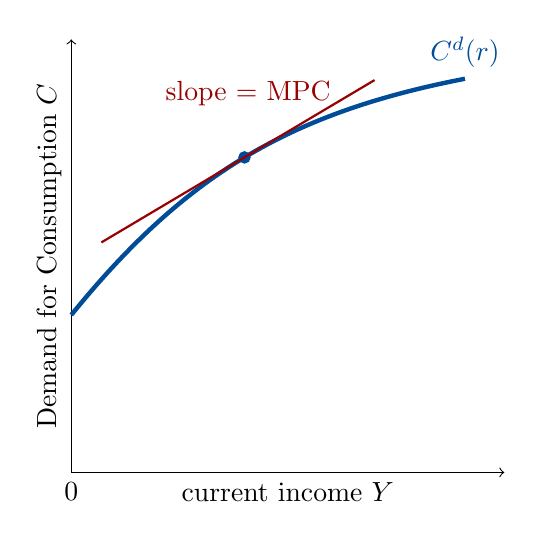
\begin{tikzpicture}
                    \pgfmathsetmacro{\x}{5};
                    \pgfmathsetmacro{\y}{5};
                    % \draw[very thin,color=gray, step=0.1] (0,0) grid (\x, \y); % gray grid
                    \draw[->] (0,0) node[below]{ $ 0 $  } -- node[below]{current income $Y$} (\x + 0.5,0) ;   % label x axis
                    \draw[->] (0,0) -- node[above, rotate=90]{Demand for Consumption $ C $} (0,\y + 0.5) ;   % label y axis
                    \draw[ultra thick, blue] (0, 2)
                        to[bend left=20]
                        node[pos=0.5,draw,fill=red,circle,inner sep=1pt] (a) {}
                        node[pos=0.51] (b) {}
                        (5, 5) node[above]{$C^{d}( r )$};
                    \draw[shorten >=-2cm, shorten <=-2cm, thick, red] (a) -- (b) node[above, yshift=.5cm]{slope $=$ MPC};
                \end{tikzpicture}
            \end{figure}
        \end{column}
        \begin{column}{0.5\textwidth}
            \textbf{Assumption C1}: demands for goods $ \uparrow  $ in income
            \begin{itemize}
                \item Recall \alert{pure income effect}
                \item Slope of tangent line is \textbf{marginal propensity to consume} (MPC)
                \begin{itemize}
                    \item what fraction of $ Y \uparrow  $ goes to $ C $?
                    \item $ MPC = d C_{D} / dY $
                \end{itemize}
                \item normal goods: both $ C $ and $ C' $ $ \uparrow  $, so saving $ S \uparrow  $
                \begin{itemize}
                    \item usually $ MPC < 1 $, i.e., not all $ Y \uparrow  $ goes to $ C $.
                \end{itemize}
            \end{itemize}
        \end{column}
    \end{columns}
\end{frame}

\begin{frame}{Current Goods Demand and Real Interest Rate}
\label{slide:Current_Goods_Demand_and_Real_Interest_Rate}
    \begin{columns}
        \begin{column}{0.5\textwidth}
            \begin{figure}
                \caption{\scriptsize Figure 11.5  Real Interest Rate $ \uparrow  $ Shifts the Demand for Consumption Goods Down}
                % \includegraphics[width=\textwidth]{<++>}
                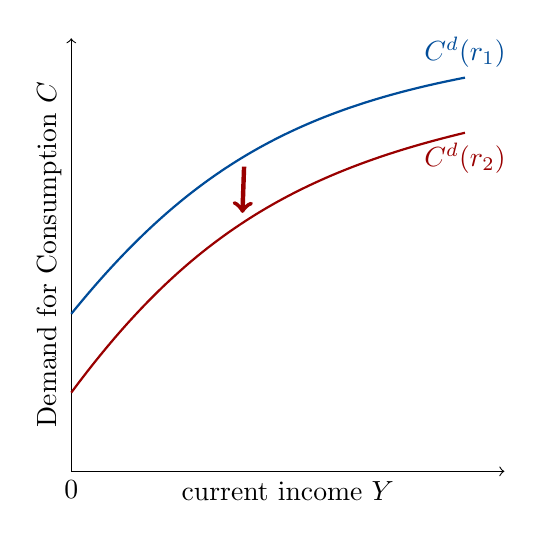
\begin{tikzpicture}
                    \pgfmathsetmacro{\x}{5};
                    \pgfmathsetmacro{\y}{5};
                    % \draw[very thin,color=gray, step=0.1] (0,0) grid (\x, \y); % gray grid
                    \draw[->] (0,0) node[below]{ $ 0 $  } -- node[below]{current income $Y$} (\x + 0.5,0) ;   % label x axis
                    \draw[->] (0,0) -- node[above, rotate=90]{Demand for Consumption $ C $} (0,\y + 0.5) ;   % label y axis
                    \draw[thick, blue] (0, 2)
                        to[bend left=20]
                        node[pos=0.5] (a) {}
                        (5, 5) node[above]{$C^{d}( r_{1} )$};
                    \draw[thick, red] (0, 1)
                        to[bend left=20]
                        node[pos=0.5] (b) {}
                        (5, 4.3) node[below]{$C^{d}( r_{2} )$};
                    \draw[ultra thick, red, ->] (a) -- (b);
                \end{tikzpicture}
            \end{figure}
        \end{column}
        \begin{column}{0.5\textwidth}
            \textbf{Assumption C2}: demands for goods $ \downarrow  $ in real interest rate
            \begin{itemize}
                \item Recall both \alert{income and substitution effect} (from dynamic model)
                \item Income effect: ambiguous (for borrowers and lenders)
                \item Substitution effect: always negative (for borrowers and lenders)
                \item \textbf{C2} assumes substitution effect dominates
            \end{itemize}
        \end{column}
    \end{columns}
\end{frame}

\begin{frame}{Current Goods Demand and Lifetime Wealth}
\label{slide:Current_Goods_Demand_and_Lifetime_Wealth}
    \begin{columns}
        \begin{column}{0.5\textwidth}
            \begin{figure}
                \caption{\scriptsize Figure 11.6  An Increase in Lifetime Wealth Shifts the Demand for Consumption Goods Up}
                % \includegraphics[width=\textwidth]{<++>}
                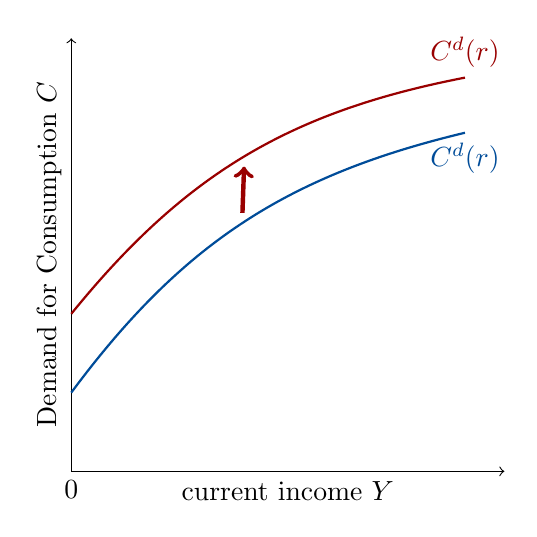
\begin{tikzpicture}
                    \pgfmathsetmacro{\x}{5};
                    \pgfmathsetmacro{\y}{5};
                    % \draw[very thin,color=gray, step=0.1] (0,0) grid (\x, \y); % gray grid
                    \draw[->] (0,0) node[below]{ $ 0 $  } -- node[below]{current income $Y$} (\x + 0.5,0) ;   % label x axis
                    \draw[->] (0,0) -- node[above, rotate=90]{Demand for Consumption $ C $} (0,\y + 0.5) ;   % label y axis
                    \draw[thick, red] (0, 2)
                        to[bend left=20]
                        node[pos=0.5] (a) {}
                        (5, 5) node[above]{$C^{d}( r )$};
                    \draw[thick, blue] (0, 1)
                        to[bend left=20]
                        node[pos=0.5] (b) {}
                        (5, 4.3) node[below]{$C^{d}( r )$};
                    \draw[ultra thick, red, ->] (b) -- (a);
                \end{tikzpicture}
            \end{figure}
        \end{column}
        \begin{column}{0.5\textwidth}
            \textbf{Assumption C3}: demands for goods $ \uparrow  $ in lifetime wealth
            \begin{itemize}
                \item similar to pure income effect
            \end{itemize}
            Note: consumer's demand is only one part of the GDP:
            %
            \begin{equation*}
               Y = C + I + G
            .\end{equation*}
            %
            We'll discuss $ I $ and $ G $ in next lecture

        \end{column}
    \end{columns}
\end{frame}

\section{Representative Firm}
\label{sec:Representative_Firm}

\begin{frame}{Overview: Firm Decision}
\label{slide:Overview__Firm_Decision}
    \begin{itemize}
        \item \textbf{production}: needs both capital $ K $ and labor $ N $, $ Y = zF( K, N ) $
        \item \textbf{endowment}: firm is endowed with initial capital $ K $
        \item \textbf{firm decision}:
        \begin{itemize}
            \item \alert{both dates}: labor ($N$), profit ($\pi$), and output ($Y$) by production
            \begin{center}
                $ \displaystyle Y = z F( K, N ) $ and $ \displaystyle Y' = z' F( K', N' ) $
            \end{center}
            \item \alert{date 0} (today): \textbf{investment} ($I$) determines future capital $ K' $ given initial capital $ K $ and \alert{depreciation rate $ \delta \in [ 0, 1 ] $},
            \begin{center}
                $ \displaystyle K' = ( 1-\delta ) K + I $
            \end{center}
        \end{itemize}
        \item \textbf{Assumptions}:
        \begin{enumerate}
            \item investment made in consumption goods
            \item remaining capital $ ( 1-\delta )K' $ liquidates tomorrow ($\because$ model ends)
        \end{enumerate}
    \end{itemize}
\end{frame}

\begin{frame}{Firm's Optimization Problem}
\label{slide:Firm_s_Optimization_Problem}
    Firm maximizes the discounted present value of profits:
    \begin{center}
        $ \displaystyle \max_{N_{D}, N'_{D}, K', I} \quad V = \pi + \frac{\pi' }{1+r} \quad \text{subject to} \quad K' = ( 1-\delta )K + I,$
    \end{center}
    where $ \pi = Y - wN - I $, and $ \pi' = Y' - w'N' + \underbrace{( 1-\delta )K'}_{\text{liquidate}} $.

    Notice: since we assume that \alert{consumer owns the firm}, so firm calculates present value using \alert{real interest rate $ r $}, i.e., how consumer discounts.

    By substituting $ \pi $, $ \pi' $, $ Y $, $ Y' $ and $ I $ into above problem, we get
    %
    \begin{equation}
    \label{eq:firm_problem}
        \begin{split}
            \max_{N_{D}, N'_{D}, K'} \quad
                & z F( K, N_{D} ) - w N_{D} - [ K' - ( 1-\delta )K ]
            \\
                & \qquad + \frac{z' F( K', N'_{D} ) - w' N'_{D} + ( 1-\delta ) K'}{1+r}
            \\
        \end{split}
    .\end{equation}
    %
\end{frame}

\begin{frame}{Firm's Optimality Conditions}
\label{slide:Firm_s_Optimality_Conditions}
    %
    \begin{align*}
        [ N_{D} ]: \quad
            & z D_{N}F( K, N_{D} ) = w
        \\
        [ N'_{D} ]: \quad
            & z' D_{N}F( K', N'_{D} ) = w'
        \\
        [ K' ]: \quad
            & -1 + \frac{z' D_{K'} F( K', N'_{D} ) + (1-\delta)}{1+r} = 0
    \end{align*}
    %
    \begin{itemize}
        \item FOCs on current and future labor are \alert{the same} as static model!
        \begin{itemize}
            \item Why? Since labor choice is \alert{static}: choose labor for \alert{current} production
        \end{itemize}
        \item FOC on future capital equalize the \alert{marginal cost and benefit} of investment
        \begin{itemize}
            \item cost: loss in current consumption (incurred today)
            \item benefit: $ \uparrow  $ in marginal production $ + $ liquidating $ K' $ (incurred tomorrow)
        \end{itemize}
    \end{itemize}
\end{frame}

\begin{frame}{Optimal Investment Schedule: Derivation}
\label{slide:Optimal_Investment_Schedule__Derivation}
    Solve for $ [ K' ] $, we get
    \begin{center}
        $ \displaystyle z' D_{K'} F( K', N'_{D} ) + 1 - \delta = 1+r \Rightarrow r = MPK' - \delta $
    \end{center}
    For consumer, there are $ 2 $ assets to undertake \alert{intertemporal substitution}:
    \begin{enumerate}
        \item saving in credit market (supply in credit mkt; demand in bond mkt)
        \item capital held by the firm for production
    \end{enumerate}
    Investing in capital means giving up (net) return $ r $ for (net) return $ MPK' - \delta $: \alert{optimal investment rule means both must offset, WHY?}
    \begin{itemize}
        \item if $ r > MPK' - \delta $: consumer will save more for bond $ \Rightarrow $ supply in credit market  $ \uparrow  $, $ r \downarrow  $
        \item if $ r < MPK' - \delta $: consumer asks firm to invest more capital $ \Rightarrow  $ $ MPK' \downarrow  $
    \end{itemize}
    To sum up, $ r = MPK' - \delta $ in equilibrium: ``optimal'' investment rule!

\end{frame}

\section{More Assumptions}
\label{sec:More_Assumptions}

\begin{frame}{Labor Demand is decreasing in $ w $ and increasing in $ z, K $}
\label{slide:Labor_Demand_is_decreasing_in___w___and_increasing_in___z__K__}
    \begin{columns}
        \begin{column}{0.5\textwidth}
            \begin{figure}
                \caption{\scriptsize Figure 11.7 The Demand Curve for $ N $ Is the Firm’s MPL Schedule}
                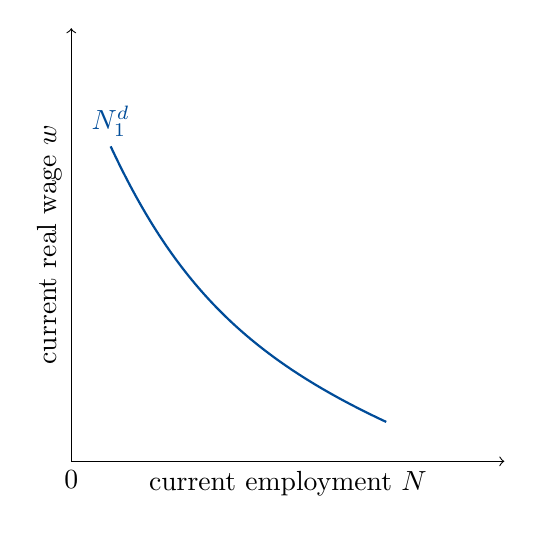
\begin{tikzpicture}
                    \pgfmathsetmacro{\x}{5};
                    \pgfmathsetmacro{\y}{5};
                    % \draw[very thin,color=gray, step=0.1] (0,0) grid (\x, \y); % gray grid
                    \draw[->] (0,0) node[below]{ $ 0 $  } -- node[below]{current employment $N$} (\x + 0.5,0) ;   % label x axis
                    \draw[->] (0,0) -- node[above, rotate=90]{current real wage $ w $} (0,\y + 0.5) ;   % label y axis
                    \draw[thick, blue]
                        (0.5, 4)
                        node[above]{$N_{1}^{d}$}
                        to[bend right=20]
                        node[pos=0.5] (a) {}
                        (4, 0.5);
                \end{tikzpicture}
            \end{figure}
        \end{column}
        \begin{column}{0.5\textwidth}
            \begin{figure}
                \caption{\scriptsize Figure 11.8  The Current Demand Curve for Labor Shifts Due to Changes in $z$ and $ K $}
                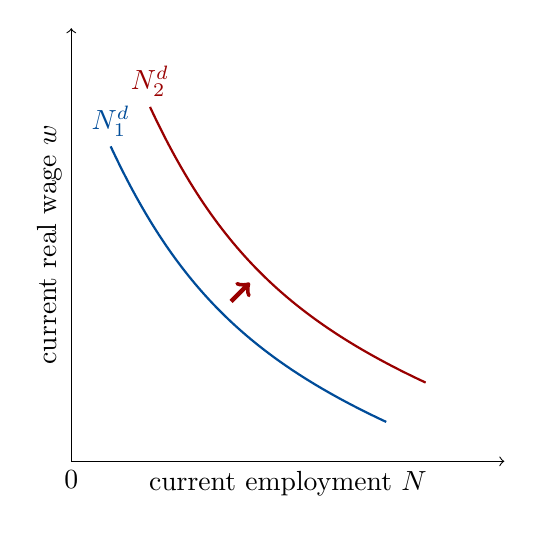
\begin{tikzpicture}
                    \pgfmathsetmacro{\x}{5};
                    \pgfmathsetmacro{\y}{5};
                    % \draw[very thin,color=gray, step=0.1] (0,0) grid (\x, \y); % gray grid
                    \draw[->] (0,0) node[below]{ $ 0 $  } -- node[below]{current employment $N$} (\x + 0.5,0) ;   % label x axis
                    \draw[->] (0,0) -- node[above, rotate=90]{current real wage $ w $} (0,\y + 0.5) ;   % label y axis
                    \draw[thick, blue]
                        (0.5, 4)
                        node[above]{$N_{1}^{d}$}
                        to[bend right=20]
                        node[pos=0.5] (a) {}
                        (4, 0.5);
                    \draw[thick, red, xshift = 0.5cm, yshift = 0.5cm]
                        (0.5, 4)
                        node[above]{$N_{2}^{d}$}
                        to[bend right=20]
                        node[pos=0.5] (b) {}
                        (4, 0.5);
                    \draw[ultra thick, red, ->] (a) -- (b);
                \end{tikzpicture}
            \end{figure}

        \end{column}
    \end{columns}
\end{frame}

\begin{frame}{Optimal Investment Schedule: Graphical Representation}
\label{slide:Optimal_Investment_Schedule__Graphical_Representation}
     \begin{columns}
         \begin{column}{0.6\textwidth}
             % \begin{figure}
                \begin{center}
                    \scriptsize Figure 11.9  Optimal Investment Schedule for the Representative Firm
                \end{center}

                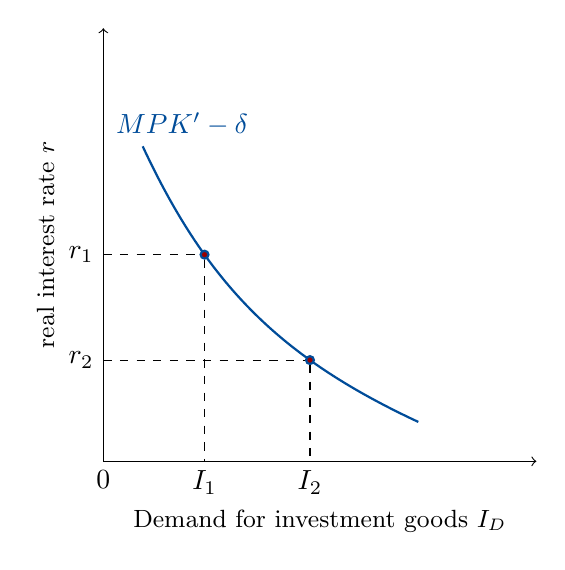
\begin{tikzpicture}
                    \pgfmathsetmacro{\x}{5};
                    \pgfmathsetmacro{\y}{5};
                    % \draw[very thin,color=gray, step=0.1] (0,0) grid (\x, \y); % gray grid
                    \draw[->] (0,0) node[below]{ $ 0 $  } -- node[below, yshift=-0.5cm]{\small Demand for investment goods $I_{D}$} (\x + 0.5,0) ;   % label x axis
                    \draw[->] (0,0) -- node[above, rotate=90, yshift=0.5cm]{\small real interest rate $ r $} (0,\y + 0.5) ;   % label y axis
                    \draw[thick, blue]
                        (0.5, 4)
                        node[above, xshift=0.5cm]{$MPK' - \delta$}
                        to[bend right=20]
                        node[pos=0.5] (a) {}
                        node[pos=0.3,draw,fill=red,circle,inner sep=1pt] (b) {}
                        node[pos=0.7,draw,fill=red,circle,inner sep=1pt] (c) {}
                        (4, 0.5);
                    \path (b); \pgfgetlastxy{\xcoord}{\ycoord};
                    \coordinate (b_x) at (\xcoord, 0);
                    \coordinate (b_y) at (0, \ycoord);
                    \path (c); \pgfgetlastxy{\xcoord}{\ycoord};
                    \coordinate (c_x) at (\xcoord, 0);
                    \coordinate (c_y) at (0, \ycoord);
                    \draw[dashed] (b_y) node[left]{$r_{1}$} -- (b) -- (b_x) node[below]{$I_{1}$};
                    \draw[dashed] (c_y) node[left]{$r_{2}$} -- (c) -- (c_x) node[below]{$I_{2}$};
                \end{tikzpicture}
             % \end{figure}
         \end{column}
         \begin{column}{0.4\textwidth}
             Put capital accumulation process into MPK and get
             $ \displaystyle z' D_{K'}F( ( 1-\delta )K + I_{D}, N'_{D} ) = r + \delta $
             \begin{itemize}
                 \item as $ r \uparrow  $, need less $ K' $ for optimal investment schedule to hold.
                 \begin{itemize}
                     \item why? diminishing MPK
                 \end{itemize}
                 \item $ K' \uparrow  $ in $ I $, so $ r \uparrow  $ also means less investment $ \Rightarrow  $ \alert{downward slope}
                 \item i.e., higher opportunity cost of investing
             \end{itemize}
         \end{column}
     \end{columns}
\end{frame}

\begin{frame}{Optimal Investment Schedule: Effect of $ K $ and $ z' $}
\label{slide:Optimal_Investment_Schedule__Effect_of___K___and___z__}
     \begin{columns}
         \begin{column}{0.6\textwidth}
             % \begin{figure}
                \begin{center}
                    \scriptsize Figure 11.10 The Optimal Investment Schedule Shifts to the Right if $K \downarrow $ or expecting $z’ \uparrow $
                \end{center}
                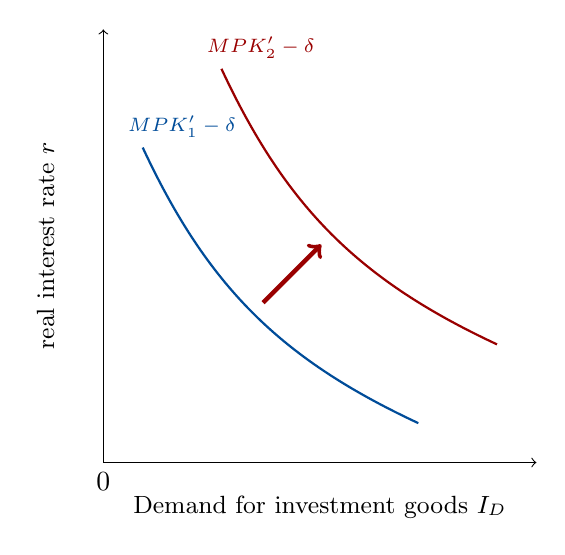
\begin{tikzpicture}
                    \pgfmathsetmacro{\x}{5};
                    \pgfmathsetmacro{\y}{5};
                    % \draw[very thin,color=gray, step=0.1] (0,0) grid (\x, \y); % gray grid
                    \draw[->] (0,0) node[below]{ $ 0 $  } -- node[below, yshift=-0.3cm]{\small Demand for investment goods $I_{D}$} (\x + 0.5,0) ;   % label x axis
                    \draw[->] (0,0) -- node[above, rotate=90, yshift=0.5cm]{\small real interest rate $ r $} (0,\y + 0.5) ;   % label y axis
                    \draw[thick, blue]
                        (0.5, 4)
                        node[above, xshift=0.5cm]{\scriptsize $MPK'_{1} - \delta$}
                        to[bend right=20]
                        node[pos=0.5] (a) {}
                        (4, 0.5);
                    \draw[thick, red, xshift=1cm, yshift=1cm]
                        (0.5, 4)
                        node[above, xshift=0.5cm]{\scriptsize $MPK'_{2} - \delta$}
                        to[bend right=20]
                        node[pos=0.5] (b) {}
                        (4, 0.5);
                    \draw[ultra thick, red, ->] (a) -- (b) ;
                \end{tikzpicture}
             % \end{figure}
         \end{column}
         \begin{column}{0.4\textwidth}
            The optimal investment schedule shifts to the right, i.e., \alert{demand for investment rises} if
            \begin{itemize}
                \item current capital $ K $ decreases:
                    $ \displaystyle \frac{d I_{D}}{d K} < 0 $
                \begin{itemize}
                    \item Intuition: need to invest more for less endowment
                \end{itemize}
                \item (expected) future TFP increases:
                    $ \displaystyle \frac{d I_{D}}{d z'} > 0 $
                \begin{itemize}
                    \item Intuition: investment is more productive
                \end{itemize}
            \end{itemize}
         \end{column}
     \end{columns}
\end{frame}

\end{document}

